\chapter{Introduction}
\label{chap: intro}
%\thispagestyle{empty}
\setcounter{page}{1}
\pagenumbering{arabic}


As humanity has continued on its journey into the future, there has been steady increase in the amount of energy used by humanity on the whole, and per capita. With this increased energy usage came a plethora of ``luxuries'' ranging from cars to computers. Many of these machines have become so essential to daily living that we forget that most of our ancestors had to live without them. Indeed, this perceived correlation between how technologically advanced a civilisation is and the amount of power it produces can be used to construct a ranking system called the ``Kardashev'' scale, where the total power produced is used as the figure of merit \cite{gray2020extended}. Taking this number to be a crude measure of the maturity of a civilisation and assuming that our civilisation wishes to become more mature, it should be clear that we should search for new energy sources enabling us to climb the ranks. More specifically, sources of energy which deplete should be phased out as we look for renewable alternatives in our quest for growth. There are only a few sources which fit the bill and are within arm's length. Nuclear fusion, the process by which lighter nuclei combine to form heavier ones, is one of these few sources, and it is also the only energy source within reach that we know exists but have not been able to harness.\footnote{One may object to this statement, by noting that there exist processes which harness energy from black holes \cite{opatrny2012black,tursunov2019fifty,comisso2021magnetic}. However, seeing that such processes shall not be realised in the foreseeable future, we ignore them here.} \par 

A second reason to investigate fusion is the more acute problem of anthropogenic climate change. The burning of fossil fuels has subjected the atmosphere of the Earth to a dramatic increase in the amount of carbon dioxide, and this carbon dioxide acts as a greenhouse gas, retaining more of the heat of the earth. The greenhouse effect, combined with many climate feedback mechanisms \cite{schneider1972cloudiness,hansen1984climate,curry1995sea,dean2018methane}, can lead to a significant increase in average temperatures and sea levels. A rise in sea levels is evidently problematic for population hubs which are close to sea, one of which being the Netherlands in which the current thesis is to be defended. Thus, a reduction in our emissions of these greenhouse gases is required, and we must turn to renewable energy sources to do so. Along with e.g. wind, solar, and fission, nuclear fusion is such a renewable energy source, and if it becomes a viable energy source in the near-future, it can aid in the energy transition. \par 

\vspace*{-2mm}
\section{A crash course in nuclear fusion}
\label{sec: chap1 motivation}

So, if nuclear fusion as an energy source is desirable, why is it not here yet? The main difficulty lies in the extreme conditions required to allow nuclear fusion to occur. This process involves fusing light atomic nuclei, with which a large amount of energy is released. In order to allow atoms to fuse one needs to overcome the Coulomb barrier, the mutual repulsion of positively charged atomic nuclei, and when the atomic nuclei are within close enough proximity the strong nuclear force binds them together. To get a feeling for the type of conditions needed to overcome this barrier, it is useful to look at a natural fusion reactor: the sun. In the fusing core of the sun, the mass density is approximately 10 times that of lead and the temperature is about 15 million degrees \textcelsius. Such conditions allow for fusion reactions such as the proton-proton chain and the carbon–nitrogen–oxygen cycle to occur \cite{bethe1939energy,salpeter1952nuclear,adelberger2011solar}. We may somewhat relax the conditions required by choosing a fusion reaction with one of the largest cross sections. \par 

On earth, then, we focus on the fusion of the deuterium and tritium isotopes of hydrogen. These fuse together to become helium and a neutron, with $17.6$ MeV of kinetic energy, i.e.
\begin{equation*}
    \ce{^{2}_{1} D} + \ce{^{3}_{1} T} \rightarrow \ce{^{4}_{2} He} + \ce{^{1}_{0} n} + 17.6 \: \mathrm{MeV}. 
\end{equation*}
To allow this fusion process to occur efficiently, the fuel must be heated to some 150 million degrees \textcelsius, and the fuel is a plasma. This hot plasma cannot be confined by means of a simple container: if the cool container wall came into contact with the hot plasma, the plasma would quickly cool. This problem may be circumvented in two manners; one can confine the fuel using its inertia (i.e. heating up the fuel on a short enough time-scale so that its inertia keeps the fuel contained), or one can confine the ionised plasma by means of magnetic fields. The current thesis focusses on the latter. \par 

The topology of the confining magnetic field is required to be of a very particular form, ultimately a consequence of the Poincar\'e-Hopf theorem \cite{hopf1927vektorfelder}, though it may be understood in simpler terms.\footnote{We shan't focus on them here but there exist fusion concepts which have differing magnetic topologies, e.g. so-called linear devices as used in gas-dynamic multiple-mirror traps \cite{burdakov2011concept,beklemishev2013novosibirsk,ivanov2017gas}, or more recent designs proposed by start-ups such as Helion \cite{waldrop2014fusion}. Although a healthy amount of scepticism is recommended for less orthodox approaches to nuclear fusion, it would be folly to categorically disregard them.} To the lowest order in the smallness of the gyroradius, charged particles stick to magnetic field lines like beads on a string. To avoid the ``beads'' being lost at the ends of the magnetic field line, one can require that the magnetic field line is in the shape of a circle so that ends do not exist. Such a {\it toroidal field component} can be achieved by bending a cylindrical solenoid into the shape of a torus. \par 
\begin{figure}
    \centering
    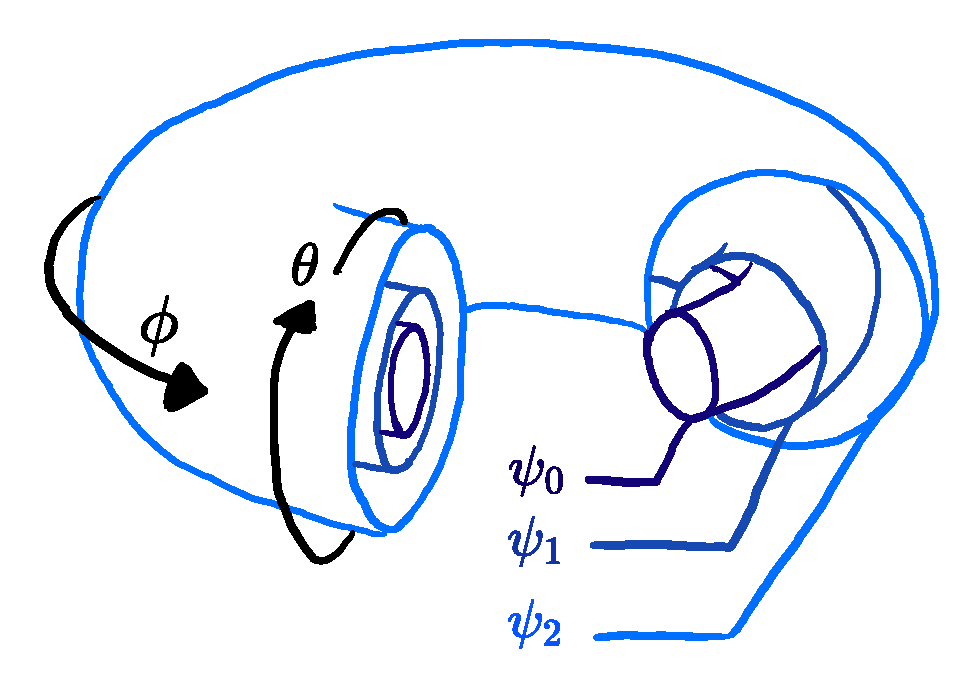
\includegraphics[width=0.6\textwidth]{3_chapters/0_introduction/img/tokamak.pdf}
    \caption{A schematic of a toroidal device. Here $\psi$ labels the various flux-surfaces, $\theta$ parameterises the poloidal angle, and $\phi$ parameterises the toroidal angle.}
    \label{fig: torus schematic}
\end{figure}
However, due to the finite gyroradius of the particles, they drift away from the field line (see \citet{de2012guiding} for expressions of this drift), and the particles ultimately end up on the reactor wall. This may be remedied by introducing a {\it poloidal field component,}, as shown explicitly in \citet{helander2014theory}, ensuring that particles stay on the magnetic field lines. In total, we thus require that the magnetic field lines go both the long (toroidally) and short way (poloidally) around the torus, and the magnetic field lines live on tori.\footnote{To be more precise, the magnetic field lines may have three distinct topologies. Firstly, the magnetic field line may loop back on itself on the torus surface, resulting in a torus knot \cite{livingston1993knot,smiet2017knots}, and such surfaces are called rational. Second, it may never loop back on itself and trace the entire surface, and such surfaces are called irrational. Lastly, the magnetic field line may fill a volume chaotically, and the magnetic field is said to be chaotic in such situations. The last of these topologies is undesirable, and we ignore such fields here.} This allows the magnetic field line, and with it the plasma, to sample the surface and equilibrate on it. The plasma on a flux surface thus has a constant pressure and temperature, and we are interested in how these vary as a function of external actuators and plasma properties. This is a ``transport problem'' of one spatial dimension; we are interested in finding how pressure and temperature depend on the flux surface label. A schematic of the geometry and typical coordinates that describe the torus is given in Fig. \ref{fig: torus schematic}.
\par 
In total we have thus found that magnetic field lines live on surfaces of tori (referred to as flux surfaces), winding both the short and long way around the torus. Each surface may then be characterised by the amount of ``twist'' of magnetic field lines on it, which is often denoted as $\iota$, the rotational transform. Quantitatively, it can be measured by following a magnetic field line of length $L$ around the torus and keeping track of the number of poloidal and toroidal turns. The rotational transform is then defined as the limit
\begin{equation}
    \iota = \lim_{L \rightarrow \infty} \frac{\textnormal{\# poloidal turns}}{\textnormal{\# toroidal turns}}.
    \label{eq: rotational transform integer definition}
\end{equation}
As stated before, inducing a toroidal component of the magnetic field can readily be achieved by bending a cylindrical solenoid into the shape of a torus. Attaining a poloidal component is less straightforward, and here we find a fork in the road that separates fusion power plant concepts.

\subsection{The tokamak}
If we assume that our toroidal field is axisymmetric, that is, the torus is invariant under toroidal rotation, there is only one way to generate the poloidal component. As one can understand from Amp\`ere's circuital law, a toroidal current provides the required poloidal component. Indeed, the \textit{tokamak} employs this method to achieve confinement and is currently the most technologically mature concept of fusion power plants. A schematic showing its essential components is provided in Fig. \ref{fig: tokamak schematic}.
\begin{figure}
    \centering
    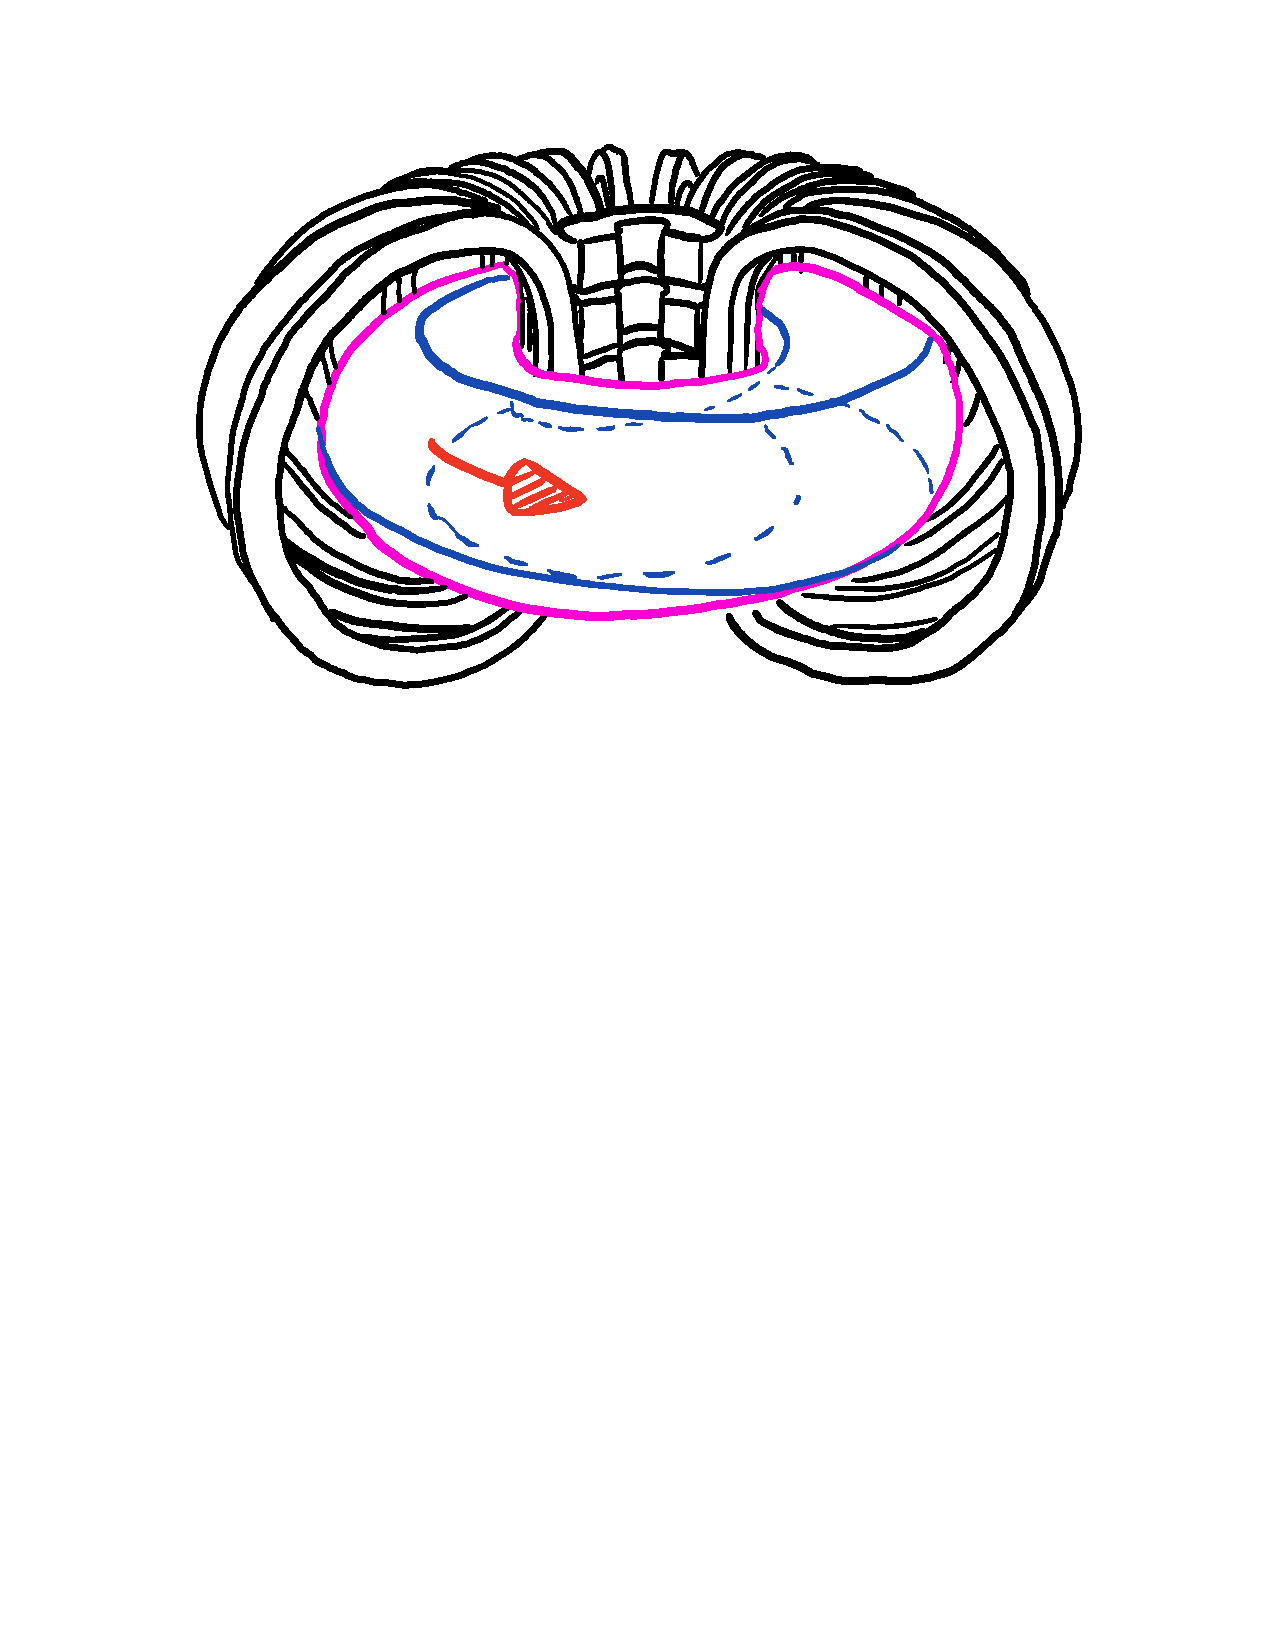
\includegraphics[width=0.5\textwidth]{3_chapters/0_introduction/img/tokamak-sketch.pdf}
    \caption{A schematic of the tokamak. In purple we see the outline of a flux-surface, in blue a field line which is situated on the flux-surface, in black we see the coils providing the necessary magnetic field, and in red we see an arrow representing the plasma current.}
    \label{fig: tokamak schematic}
\end{figure}
\par 
After its inception in 1950 in the U.S.S.R. by Andrei D. Sakharov and Igor E. Tamm, the tokamak made large strides in the late 1960s with the T-3A experiment reaching temperatures 10 times that of any other fusion power plant concept \cite{azizov2012tokamaks}. This solidified the tokamak's position as the leading concept, and we still feel the reverberations. Although the tokamak does have a number of advantages, it also suffers from problems that must be taken seriously. For example, in tokamaks a violent instability can arise, called a disruption, and in full-scale reactors it may irreparably break the device. The source of this Achilles' heel is the large current required to generate the poloidal magnetic field, and many are considering current-free alternatives to the tokamak.

\subsection{The stellarator}
The \textit{stellarator} provides this current-free path to confinement and has a more stable equilibrium without interruptions. The requirement of a current-free device necessitates that the torus is three-dimensional, in order to have rotational transform. As shown by \citet{mercier1964equilibrium}, one can generate a rotational transform by having current, ellipsoidally shaped cross sections which rotate as one travels toroidally around the torus, and by having torsion of the magnetic axis. The first solution is the one employed by the tokamak, and the latter two nonaxisymmetric solutions by the stellarator, and a sketch of the stellarator may be found in Fig. \ref{fig: sketch stellarator}. \par

The stellarator was first proposed in 1951 by Lyman Spitzer Jr. (head of the Princeton Astrophysics Department in New Jersey, U.S.A. at the time), only one year after the tokamak \cite{spitzer1951project}. Despite the fact that the dates of birth of the stellarator and the tokamak are fairly close, the stellarator has historically underperformed on measures such as energy confinement time, a typical time scale on which the plasma loses energy to its environment \cite{sudo1990scalings,stroth1996energy,sunn2017key}. One reason for this poor performance compared with tokamaks is the large configuration space of stellarators. \citet{boozer2005physics} estimates that the shape of stellarators may be parameterised by some 50 free parameters (which may be contrasted with tokamaks having roughly 4). If we discretise this space by using 10 nodes per parameter, the space consists of $10^{50}$ stellarators, roughly the number of atoms that comprise the earth. These stellarators have large differences in energy confinement times, and in 1951 the theoretical and numerical tools to navigate this space were not available. With the advent of supercomputing and novel theoretical models, it became feasible to explore this large space \cite{catto1981omnigenous,boozer1983transport,beidler1990physics,grieger1992physics,grieger1992modular,nuhrenberg1995overview}, allowing one to optimise for a number of criteria and find candidate stellarators with attractive properties. \par

Wendelstein 7-X (W7-X), the world's largest stellarator situated in Germany, is such an optimised stellarator, and it has shown the best fusion performance of any stellarator plasma to date \cite{wolf2017major,wolf2019performance}. \citet{beidler2021demonstration} showed that these records were enabled by the W7-X optimisation, highlighting its potential. Since the design of W7-X, many novel optimisation codes and methods have been developed \cite{wagner1998stellarators,spong2001physics,kovari2014process,kovari2016process,drevlak2018optimisation,dudt2020desc,landreman2021simsopt,mcgreivy2021optimized}. This has made it possible to optimise for a large number of criteria, such as minimal fast particle losses, satisfying certain engineering constraints, and, importantly for the current thesis, low heat losses due to micro-turbulence.

\begin{figure}
    \centering
    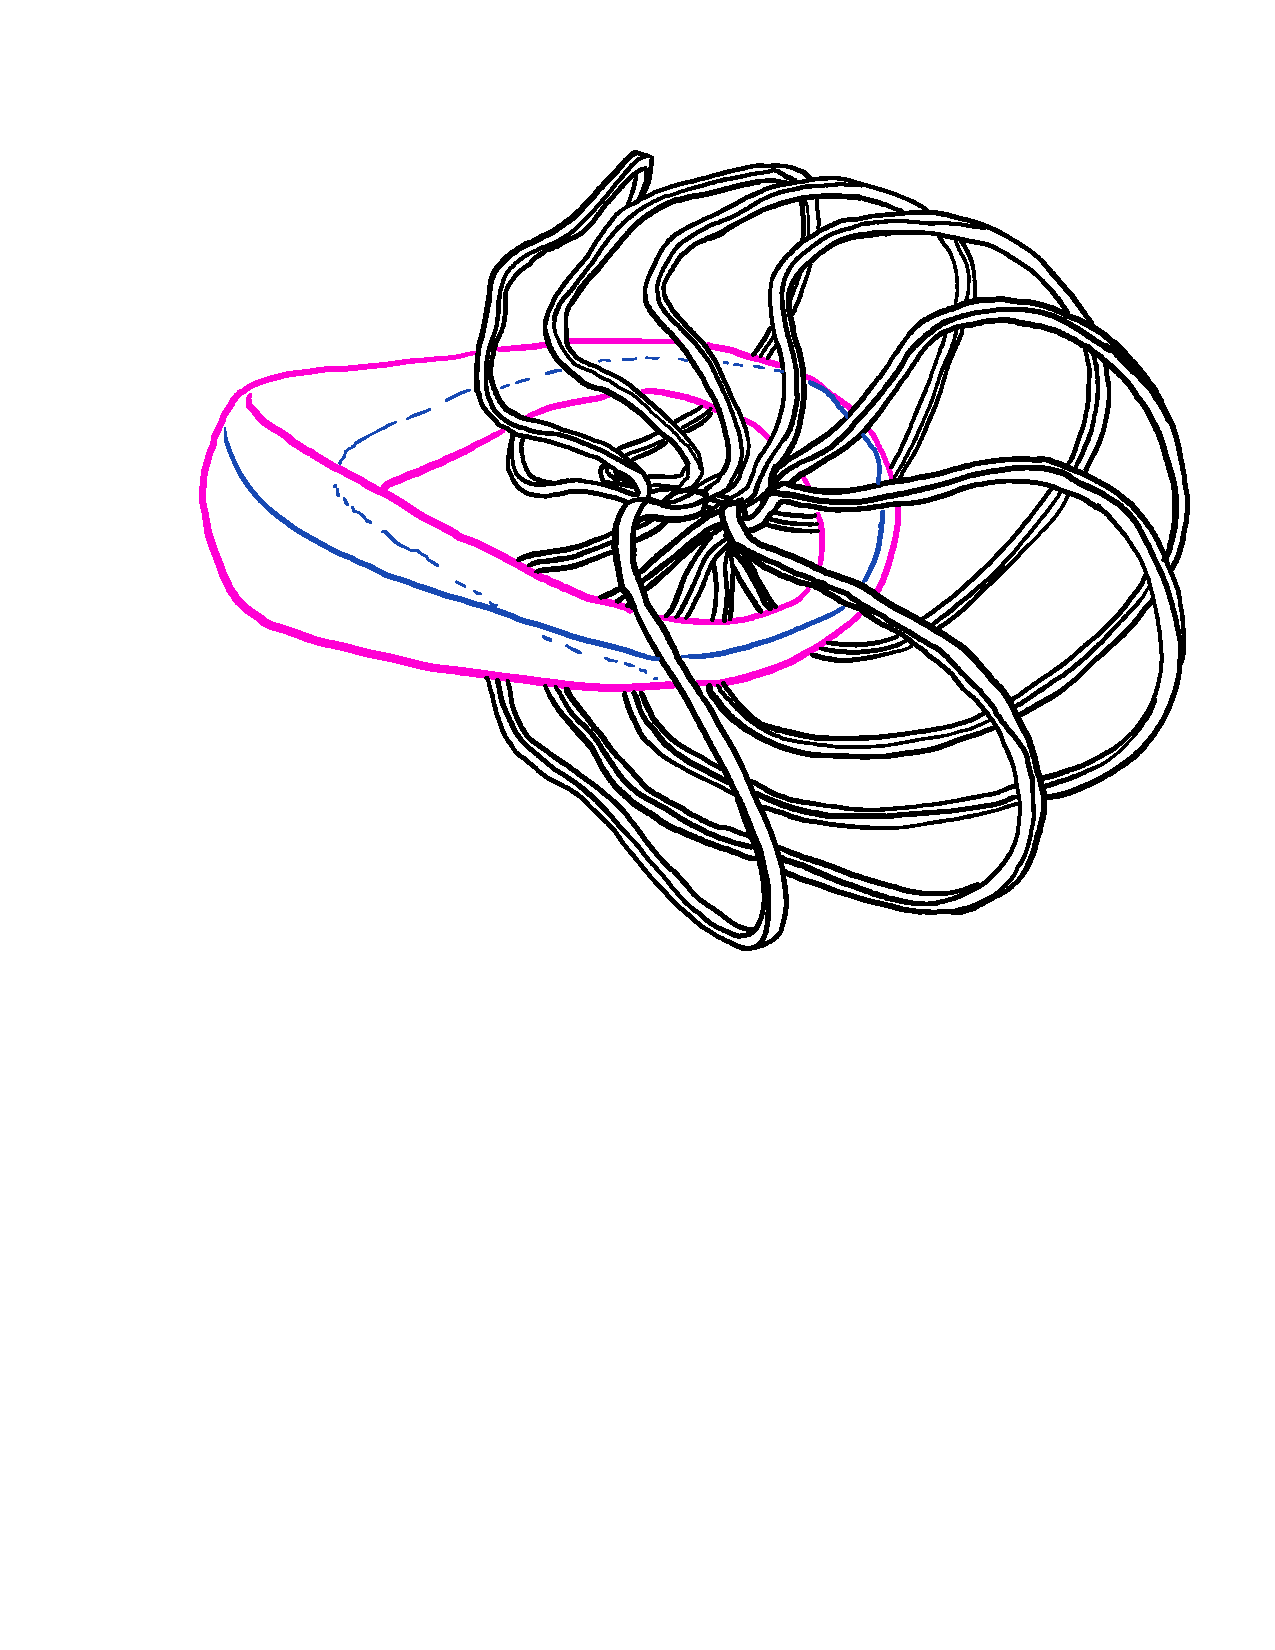
\includegraphics[width=0.6\textwidth]{3_chapters/0_introduction/img/stellarator-sketch.pdf}
    \caption{A sketch of a stellarator with half of all the coils drawn in black, the flux surface in purple, and a magnetic field line in blue. It can be seen that the complex three-dimensional shape can be achieved by having non-planar coils, which need to be constructed within tight tolerances. Based on \citet{wechsung2022precise}.}
    \label{fig: sketch stellarator}
\end{figure}



\section{Micro in scale, macro in consequences}
\label{sec: chap1 background}
Micro turbulence refers to turbulence that takes place on the scale of the gyroradius, which in tokamaks and stellarators is on the order of centimetres. Compared to the size of the device itself (typically measured in metres), this scale is indeed small. However, such smallness does not imply that one can safely ignore it.  Indeed, this microscopic turbulence is the main contributor to heat loss in current tokamaks and optimised stellarators, and we ought to understand it better if we are to make nuclear fusion power plants a reality. \par  

To deepen our understanding, we make a distinction between two types of transport which are relevant in magnetic confinement devices, neoclassical transport and turbulent transport, and the former can play an important role in some situations. There are many accounts available on neoclassical transport \cite{galeev1979reviews,kovrizhnykh1984energy,mynick2006transport,freidberg2008plasma,beidler2011benchmarking,wesson2011tokamaks}, and therefore we shall only focus on the high-level understanding. A further distinction is made between neoclassical transport in stellarators and tokamaks, as they can be quite distinct. Let us start by focussing on the latter.

\subsection{Neoclassical transport in tokamaks}
To make statements about transport, it is useful to quantify it by means of a diffusion coefficient, denoted as $D$. This coefficient of some Brownian ``random walk'' process may be estimated as
\begin{equation*}
    D = \Delta r^2/\tau,
\end{equation*}
where $\tau$ is a typical timescale at which steps of the random walk are taken, and $\Delta r$ is the step-size of the walk. A simple estimate of this diffusion coefficient for a magnetised plasma can be derived in the following manner. \par 
The typical step-size perpendicular to the field will be the gyroradius $\rho$, and the time scale at which such steps are taken is the collision frequency. Focussing on energy transport, collisions of particles with similar mass lead to this transport.\footnote{This may be verified by investigating the limit case where one particle is much heavier than the other one. This scenario is like throwing a tennis ball against a wall; the tennis ball imparts a negligible amount of energy to the wall.} Let us estimate this collision frequency as follows; for Coulomb interactions to affect the particle trajectory, the kinetic and Coulomb energy should be of similar magnitude, i.e.
\begin{equation*}
    \frac{E_{\rm C}}{E_{\rm kinetic}} = \frac{\frac{1}{4\pi \epsilon_0} \frac{(Ze)^2}{r_{\rm C}} }{\frac{1}{2} m v^2} \approx 1 \implies r_{\rm C} \approx \frac{(Ze)^2}{2 \pi \epsilon_0 m v^2},
\end{equation*}
with $e$ being the elementary charge, and $Z$ the charge number. Therefore, if the particles come within a distance $r_{\rm C}$ of each other, the Coulomb potential can significantly alter the trajectory. Now, the collision frequency may be estimated as $\nu_{\rm C} \sim n \pi r_{\rm C}^2 v$, and taking the velocity to be thermal ($v \sim \sqrt{T/m}$) we find
\begin{equation*}
    \tau_{\rm C} \sim  \frac{1}{\nu_{\rm C}} \sim \frac{\epsilon_0^2 m^{1/2} T^{3/2}}{n (Ze)^2}.
\end{equation*}
Let us combine the gyroradius and collision time to estimate the diffusion coefficient
\begin{equation}
    D_{\rm C} = \frac{\rho^2}{\tau_{\rm C}} \sim \frac{n}{\epsilon_0^2 B^2} \sqrt{\frac{m}{T}},
\end{equation}
and the scaling with mass implies that ions will be the dominant contributor to energy transport. A rigorous derivation is given by \citet{braginskii1958transport}, giving rise to the same scaling. Using typical values for the various parameters, one finds $D_{\rm C} \approx 10^{-3} \: {\rm m^2/s}$ \cite[p.~465]{freidberg2008plasma}. \par 
This classical estimate of heat diffusion is too optimistic, however, as step size and collision frequency increase in toroidal devices \cite[Ch.~7]{helander2005collisional}. Although the precise increase, in general, depends on the magnitude of the collision frequency \cite{hinton1976theory}, we focus on the low-collisionality limit here (which holds for a sufficiently high temperature, as desired in a future fusion reactor). In this limit, the diffusion coefficient increases due to trapped particles. Such particles are trapped in regions of weak magnetic field strength, which may be seen as follows. The energy of a particle is equal to
\begin{equation}
    E = \frac{1}{2}mv_\parallel^2 +  \mu B \implies v_\parallel = \pm \sqrt{\frac{2}{m}}\sqrt{E - \mu B}
    \label{eq: v par}
\end{equation}
where $\mu$ is the magnetic moment $\mu = mv_\perp^2/2B$, and the parallel and perpendicular symbols refer to the orientation with respect to the magnetic field. The magnetic moment is conserved for charged particles in magnetic fields \cite{littlejohn1983variational}, and thus the particles are restricted to reside in regions that satisfy $E - \mu B > 0$. If there exists a $B$ on the flux surface such that $B > E/\mu $, a particle is said to be trapped. \par
These particles make a radial excursion away from the flux surfaces by a ``banana width'' $\Delta r_{\rm b} \sim (\rho / \iota)\cdot \sqrt{R_0/a} $, with $a$ and $R_0$ being the minor and major radius of the torus, respectively. The collision time is reduced since changing the trajectory from trapped to untrapped is sufficient to make a step of a banana width (i.e. a small change in $v_\parallel$ is sufficient to make this step). This may be seen as follows; the parallel velocity as given in Eq. \eqref{eq: v par} goes as $v_\parallel \sim \sqrt{1-\mu B/E}$. Realise that the most deeply trapped particles have $v_\parallel=0$, and shallowly trapped particles have $E=\mu B_{\rm max} \implies \mu =E / B_{\rm max}$. In the latter case, the parallel velocity goes as $v_\parallel \sim \sqrt{(B_{\rm max} - B)/B_{\rm max}}\sim \sqrt{\delta B/B_{\rm max}}$ and this variation in the magnetic field goes as $\delta B/B \sim a/R_0$. Therefore, changing $(v_\parallel/v)^2$ by a factor $\epsilon$ is sufficient, and the collision time changes by a factor $\tau_{\rm b} = \tau_{\rm C} \cdot (a/R_0)$  \cite{helander2005collisional}. The diffusion coefficient decreases somewhat due to the fact that only trapped particles contribute to it, reducing it by a factor $\sqrt{2 a /R_0}$. All in all, one finds that this neoclassical estimate of the diffusion coefficient, which accounts for the trapped particles, is
\begin{equation}
    D_{\rm b} \sim \frac{(R_0/a)^{3/2}\sqrt{2} }{\iota^2} D_{\rm C},
\end{equation}
where the prefactor to $D_{\rm C}$ is of order $100$. Taking into account this trapped particle behaviour, we thus find $D_{\rm b} \approx 10^{-1} \: {\rm m^2/s}$. Although this neoclassical transport in tokamaks is generally much too low to explain what is observed in experiments, and it is found that turbulent transport is dominant instead, in classical stellarators (i.e. stellarators that are not optimised), neoclassical transport can pose a severe hindrance to confinement.

\subsection{Neoclassical transport in stellarators}
In general (unoptimized) stellarators, the dominant neoclassical transport is (like in tokamaks) due to trapped particles, if the collision frequency is small enough. However, the problem is exacerbated in stellarators, as trapped particles can drift across flux surfaces, transporting the particles and heat across the device. Tokamaks do not suffer from this problem, as their axisymmetry automatically implies that trapped particles do not drift radially on average, a result often called \textit{Tamm's theorem.} \par 
In terms of a diffusion coefficient, it is useful to realise that the radial drift scales as $\boldsymbol{v}_D \cdot \nabla r \sim \hat{r} \cdot  T/Ze B$, where $\hat{r}$ measures how much the trapped particles are drifting radially on average, and one can construct an estimate (see Ref. \cite{helander2012stellarator}). In terms of collision time, a small change in the parallel velocity can change the orbit from trapped to untrapped, significantly altering the trajectory. To this end, we introduce $\tau_{\rm s} \sim \tau_{\rm C} \cdot \epsilon_{h}$ where $\epsilon_{h}$ measures the variation of the magnetic field, $\epsilon_{h} \sim \delta B/ B$ (e.g. in the tokamak case we found $\delta B/B \sim a/R_0$). The diffusion coefficient is again decreased by a factor $\sqrt{\epsilon_{h}}$ due to the trapping fraction, and, in total, we find that this coefficient becomes\footnote{This estimate is too pessimistic, as the higher thermal velocity of electrons as compared to ions results in a charge imbalance, giving rise to an electric field. This electric field will cause the particles to precess around the flux surface, which reduces the radial drift they experience. Consequently, the diffusion coefficient decreases with such an electric field (see e.g. \citet{beidler2011benchmarking}). We ignore this effect here.}
\begin{equation}
\begin{aligned}
    D_{\rm s} \sim v_D^2 \tau_{\rm s} \sqrt{\epsilon_{h}} & \sim \left( \epsilon_{h}^{3/2} \hat{r}^2 \right) \times \frac{\epsilon_0^2 m^{1/2} T^{7/2}}{n (Ze)^4 B^2}  \\
    &\sim  \epsilon_{\rm eff}^{3/2} \times \frac{\epsilon_0^2 m^{1/2} T^{7/2}}{n (Ze)^4 B^2},
\end{aligned}
\end{equation}
where we have define the factor in brackets as $\epsilon_{\rm eff}^{3/2}$. Notice the strong dependence on temperature, where increasing the temperature greatly increases the diffusion coefficient. However, we have the freedom to change the geometry of the magnetic field, thereby reducing $\epsilon_{\rm eff}$ and decreasing the radial drift experienced by the trapped particles. Ideally, we wish to find stellarators in which trapped particles experience zero average radial drift, and in such cases $\epsilon_{\rm eff}$ is exactly zero as well. Note that this does not mean that the diffusion coefficient will vanish too; one should revert to an argument like the tokamak case if the trapped particles do not drift radially on average.
\par 
It is in attaining the favourable property of radially stationary trapped particles that we find fundamental topics in stellarator physics. Indeed, the work is so central to the field that its pioneers, Allen Boozer and J\"urgen N\"uhrenberg, were awarded the Hannes Alfv\'en Prize in 2010 for their contributions made \cite{mendoncca201037th}. The findings enabled the community to reduce the neoclassical transport in stellarators to levels comparable to those of a tokamak \cite{landreman2022magnetic,paul2022energetic,goodman2022constructing}, and this reduced neoclassical transport has resulted in greatly improved performance in stellarators (see, e.g. Ref. \cite{beidler2021demonstration}). With neoclassical transport levels comparable to those of tokamaks, a different transport mechanism is dominant: turbulent transport.

\subsection{Turbulent transport}
\begin{figure}[!b]
  \centering
  \subfloat[Prior to H-mode]{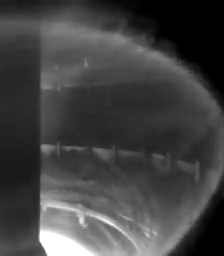
\includegraphics[width=0.4\textwidth]{3_chapters/0_introduction/img/pre-H-mode.png}}
  \hfill
  \subfloat[In H-mode]{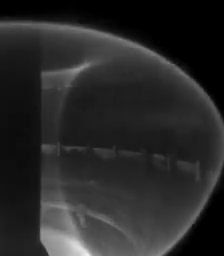
\includegraphics[width=0.4\textwidth]{3_chapters/0_introduction/img/H-mode.png}}
  \caption{The MAST tokamak prior to and in H-mode. Taken from shot \#29742 of the M9 campaign. One can see that the plasma shows fewer filaments and a more smooth, stable flux-surface in H-mode.}
  \label{fig: L-H mode in MAST}
\end{figure}
In tokamaks and stellarators with little neoclassical transport, the step size is not determined by the gyroradius alone, but by turbulent fluctuations in the electric field as well.\footnote{Fluctuations in the magnetic field contribute too, but we ignore such effects here. We also stress that a random-walk model is not always appropriate for turbulence, see e.g. \cite{del2005nondiffusive,mier2008characterization,del2010non,dif2010validity,nastac2022stochastic}} These fluctuations arise because of instabilities, which are driven by the free energy in the gradient. Turbulent fluctuations will cause the particles to be pushed around, causing them to be transported across flux surfaces, and we may estimate its magnitude as follows. The drift velocity of particles due to an electric field can be estimated as $v_E \sim \nabla \phi/B$, where the electric potential satisfies $\boldsymbol{E} = - \nabla \phi$. If we then impose that the transport is local (i.e., it takes place on the scale of the gyroradius and is thus micro-turbulence), the step size and spatial variation in $\phi$ are of order $\rho$, resulting in
\begin{equation}
    D_{\rm turb} \sim \frac{\rho \nabla \phi}{B} \sim \frac{T}{ZeB} \times \left( \frac{Ze\phi}{T} \right).
\end{equation}
The factor in brackets denotes the ratio of the potential energy of the particle to the temperature, and this electrostatic potential is determined by the turbulence. Its dependencies are crucial to understanding how transport in turbulent systems behaves, and the main idea of this thesis is to find a method of estimating the magnitude of this quantity. To put a number on this turbulent transport, in experiments it is typically found that $D \approx 1 \: {\rm m^2/s}$, roughly an order of magnitude higher than our estimate using trapped particles in tokamaks.
\par 

To sketch the effects this increased diffusion coefficient has on the performance of our reactor, one can investigate situations in which this anomalous transport is largely suppressed. In tokamaks, this is the case in the so-called H-modes, in which there exists a steep pressure gradient at the edge of the reactor \cite{itoh1988model,burrell1992physics,groebner1993emerging,burrell2005advances}. Such an H-mode is characterised by a reduction in transport, making it possible to maintain a steep pressure gradient. This reduction in transport brings with it such benefits that many tokamak power plant scenarios now assume H-mode operation to achieve the conditions required. A figure showing the transition to H-mode in MAST is shown in Fig. \ref{fig: L-H mode in MAST}. \par 

As we have seen, a deeper understanding of micro-turbulence is highly sought after as it may help us reach improved reactor performance. This is true for both tokamaks and stellarators, where the latter have a much larger configuration space, which may help in reaching reduced micro-turbulence. However, since the flowing plasma creates electromagnetic fields affecting its own flow, the process is nonlinear. In a mathematical sense, this disallows us from decomposing the solution space into simpler independent constituents (e.g. Green's functions or Fourier modes), hindering analysis. Physically, this non-linear behaviour manifests itself as multiple instabilities that interact with each other, which can cause predator-prey-like dynamics \cite{morel2013characterization}. In tokamaks and stellarators the turbulence is well described by the gyrokinetic equations, and these equations take centre stage for micro-turbulence investigations.

\subsection{The gyrokinetic equations}
\label{subsec: Gyrokinetic equations}
There exist a number of resources that derive the gyrokinetic equations in different ways \cite{dubin1983nonlinear,hahm1988nonlinear,brizard2007foundations,parra2011phase,krommes2012gyrokinetic,burby2015hamiltonian}, and we shall not focus too much on such specifics here and instead focus on the main concepts and difficulties involved. In general, in plasma kinetics one is interested in solving a Boltzmann equation (which is a continuity equation) of the form
\begin{equation}
    \frac{\mathrm{d} f_s}{\mathrm{d} t} \equiv \frac{\partial f_s}{\partial t} + \boldsymbol{v} \cdot \nabla_{\boldsymbol{r}} f_s + \frac{\boldsymbol{F}}{m} \cdot \nabla_{\boldsymbol{v}} f_s = \mathrm{sources/sinks/collisions},
\end{equation}
where $f_s(t,\boldsymbol{r},\boldsymbol{v})$ is the plasma distribution function of species $s$, $t$ is the time, $\boldsymbol{r}$ is the position vector, $\boldsymbol{v}$ is the velocity vector, $\boldsymbol{F}$ is the force acting on the particles, and we have made use of Feynman subscript notation for the divergence. The right-hand side of the above equation encapsulates the sources and sinks of particles, energy, or momentum, which may consist of collisions with other species and external actuators. \par 

In fusion-relevant conditions, the electromagnetic force typically dominates, meaning that one may take the Lorentz force
\begin{equation}
    \boldsymbol{F} = q \left( \boldsymbol{E} + \boldsymbol{v} \times \boldsymbol{B} \right).
\end{equation}
It is crucial to realise that a non-linearity enters here: since the plasma consists of charged particles, it generates its own electromagnetic fields, making $\boldsymbol{E}$ and $\boldsymbol{B}$ dependent on $f$. This non-linearity hinders straightforward mathematical analysis. We are somewhat helped by the fact that, under fusion-relevant conditions, collisions can often be neglected, as the collision frequency scales as $T^{-3/2}$, with $T$ being the plasma temperature. Hence, at the extreme temperatures present in fusion-relevant conditions, collisions become rare and may be neglected,\footnote{An excellent counter-point is that, if collisions are negligible, how is fusion to happen? More formally, it turns out to be a matter of time scales, i.e. collisions happen much less often than typical frequencies associated with the micro-turbulence and the turbulence can saturate without feeling the effects of the collisions \cite{garbet2010gyrokinetic}. However, this assumption is not always valid and collisions affect turbulence in some situations \cite{rewoldt1990toroidal,lin1999effects,falchetto2004effect,morren2022influence}. In certain systems, important differences can arise if one takes the collisionless limit instead of neglecting collisions all together, essentially due to the mathematical fact that $\lim_{\mathrm{x \rightarrow a}} f(x) \neq f(a)$ in general: see \citet{ng2021landau} for a pertinent example.} rendering this equation somewhat simpler. Other sources and sinks (e.g. electron cyclotron resonance heating or pellet injection) should in general be taken into account but are ignored here. \par

This simplified form with neglected collisions, sources, and sinks is called the \textit{Vlasov equation,} and it has several properties of interest. Importantly, the Vlasov equation has a Liouville theorem (i.e., phase-space flow incompressibility) and an action principle for both electromagnetic fields and particles \cite{landau2013classical}. We may simplify this action once more by expanding the Vlasov equation around a small parameter $\delta$, where $\rho/L\sim \omega/\Omega_{\rm ions} \sim Ze \phi / T \sim \delta $, with $L$ denoting a global length scale (e.g. minor radius), $\omega$ denoting frequencies of interest and $\Omega_{\rm ions}$ denoting the ion gyration frequency. This expansion, combined with the gauge freedom of the action, allows us to find a reduced set of equations (see \citet{scott2017gyrokinetic}). The resulting reduced set of equations is the gyrokinetic equations and its phase-space dimensionality is lower one degree lower than the Vlasov equation (i.e. 5 dimensions instead of 6). The ``neglected'' dimension turns out to be the so-called gyrophase, the phase of a particle gyrating around a magnetic field line (a sketch may be seen in Fig. \ref{fig: gyrophase sketch}). The reason why it may be neglected makes physical sense as well: in the limit of strong magnetic fields where $\omega/\Omega_{\rm ions} \sim \delta$, the gyration frequency is much larger than other time scales of relevance, meaning that it can be safely ignored. \par
\begin{figure}
    \centering
    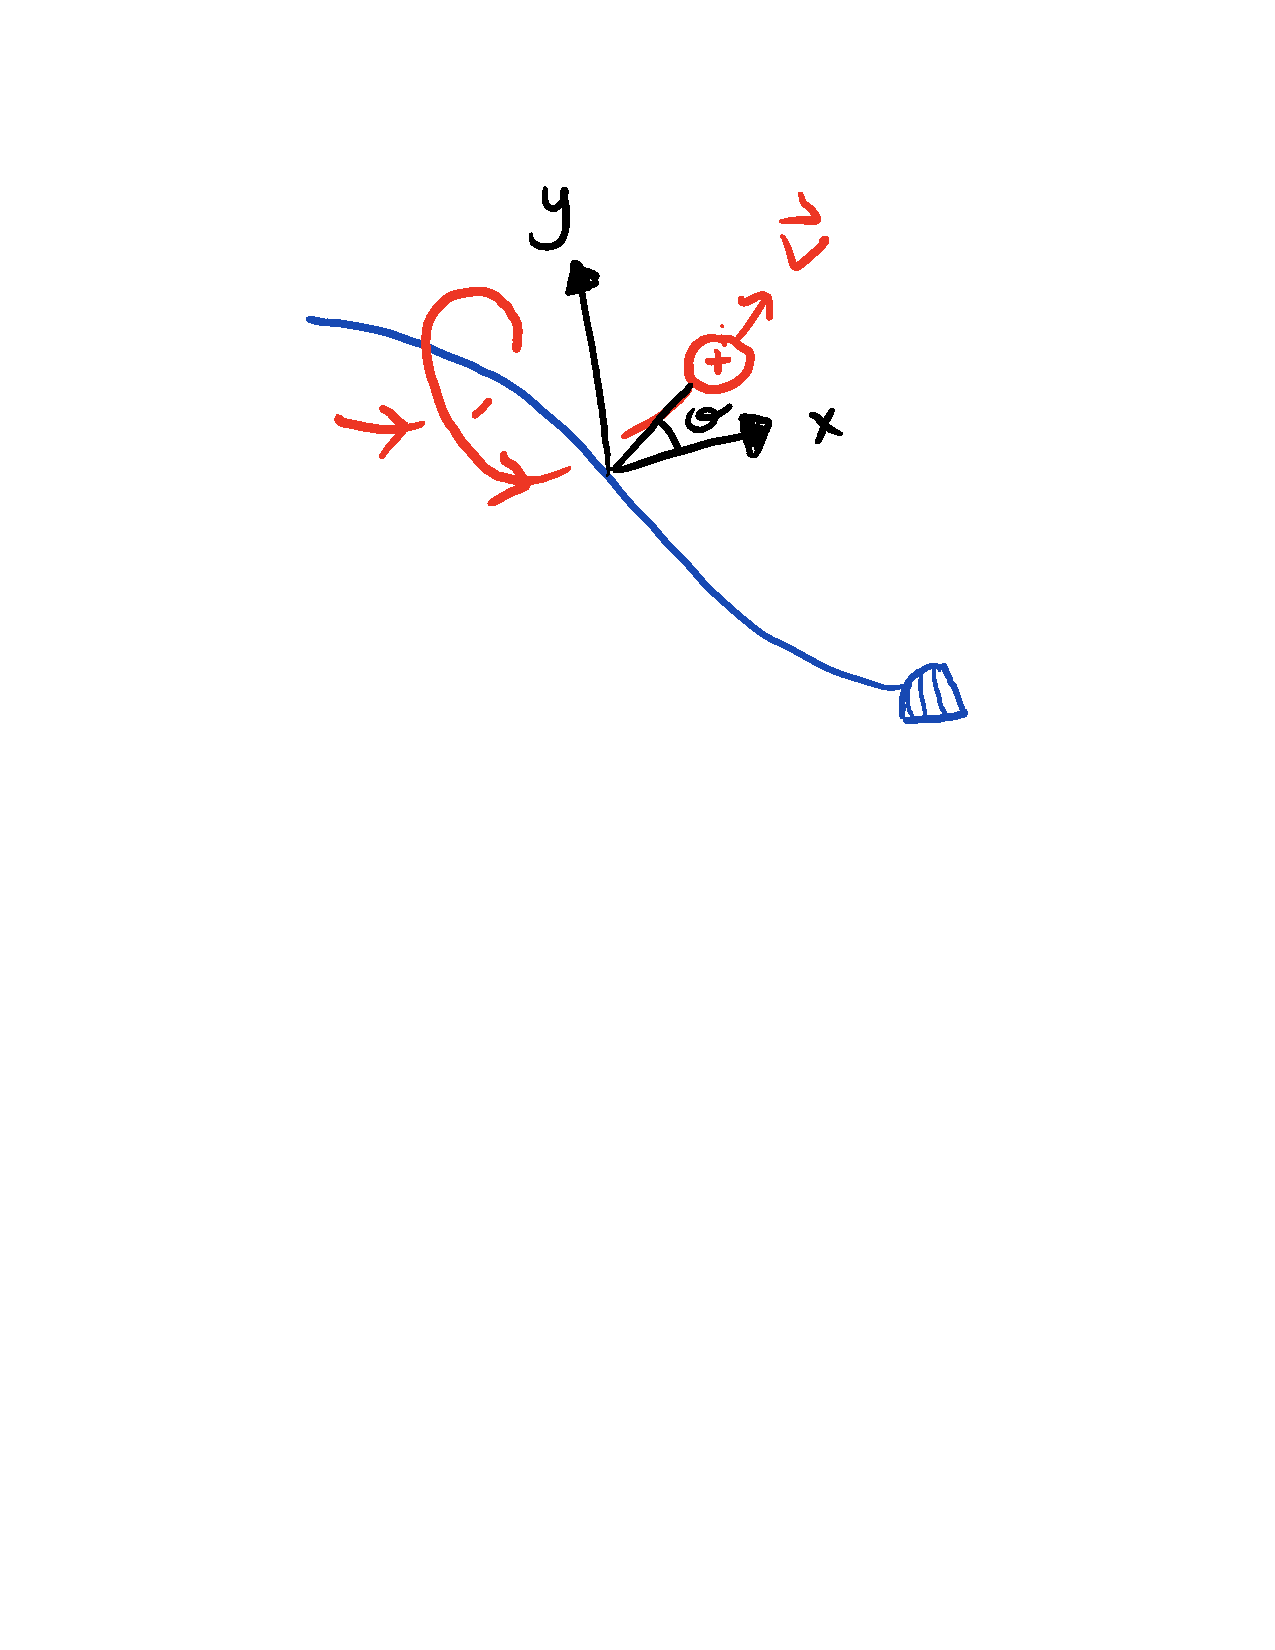
\includegraphics[width=0.5\textwidth]{3_chapters/0_introduction/img/gyrophase-sketch.pdf}
    \caption{A sketch of a positively charged particle's path in red, as it gyrates around a magnetic field line in blue. The helical path has a certain gyrophase associated with it at every location, denoted as $\vartheta$.}
    \label{fig: gyrophase sketch}
\end{figure}

Although this set of equations constitutes a reduced model, it is still computationally very demanding to solve. There are multiple codes available which solve these equations (where some use various additional assumptions on the magnetic geometry; see Refs. \cite{jenko2000electron,barnes_michael_2022_6882296,maurer2020gene,barnes2019stella,francisquez2020gkeyll} for a non-exhaustive list), but computations can still typically take $\gtrsim 10^5$ CPU-hours.\footnote{It should be noted that this is a rapidly evolving field, with large strides being made by the year. For example, by using fully spectral methods on GPUs certain calculations have been cut down by orders of magnitude \cite{mandell_dorland_landreman_2018,mandell2022gx}.} Millions of lines of code (a count of a couple codes brings me to a total of 2288153 lines) and some hundred thousand man-hours have been put into this development, and the extremely thorough numerical analysis by the community has brought with it great insight. One particularly pressing insight is that when equilibrium parameters are changed slightly (e.g., magnetic shear, ratio of thermal to magnetic pressure, geometry), the micro-turbulence may change greatly \cite{dimits2000comparisons,kinsey2006effect,alcuson2020suppression,volvcokas2022ultra,mulholland2023enhanced}. As such, each new point in parameter space should be carefully simulated before we can make statements about them. This raises the question: is there anything we can say about these equations {\it in general?} Are there fundamental properties of the Vlasov and gyrokinetic equations that can estimate the magnitude of turbulence?

\section{Available energy}
There are indeed fundamental properties that one can exploit to make general statements if the system is Hamiltonian and thus satisfies Liouville's theorem. This boils down to the fact that the dynamics of such a system inhabits a constrained subspace in the set of all distribution functions. The set of accessible distribution functions is set by the initial distribution function $f_i \equiv f(t=0)$, and we denote the total set $\mathcal{F}_L$ (where the subscript denotes that the space is constrained via Liouville's theorem) as
\begin{equation}
    f(\boldsymbol{x},t) \in \mathcal{F}_L [f_i]; \; \forall t \geq 0.
    \label{eq:set-of-all-distribution-functions}
\end{equation}
We may furthermore associate a total thermal energy to each distribution function, which is simply
\begin{equation}
    E_T[f] \equiv \int \epsilon f(\boldsymbol{x},t) \mathrm{d} \boldsymbol{x},
\end{equation}
where $\epsilon$ is the particle energy (typically $\epsilon=mv^2/2$).\par 
A natural question to ask oneself given these concepts is the following: \textit{what is the minimiser of the thermal energy in the set of accessible distribution functions?} In a more mathematical sense, we wish to find the function $f_g$ (sometimes denoted as $f_0$), which satisfies
\begin{equation}
    f_g \equiv \argmin_{f \in \mathcal{F}_L[f_i]} \:  E_T[f].
\end{equation}
This minimiser of thermal energy is called the ground state $f_g$, and this quantity will play a central role in the current thesis. It is a quantity of relevance because the Vlasov equation (for certain boundary conditions) conserves the total energy, which is the sum of the energy in the electromagnetic field and the thermal energy. Therefore, if one loses thermal energy, this energy has to be transferred to the electromagnetic field, which, in turn, may drive instabilities. If we start with an initial state $f_i$ in which there is no energy in the electromagnetic field, we can thus construct an upper bound for the total energy that can possibly reside there. It is this upper bound that we shall call the \textit{available energy}, which shall be abbreviated to \AE{}, and it is formally defined as
\begin{equation}
    A = E_T[f_i] - E_T[f_g] \geq 0,
\end{equation}
where the available energy $A$ is always greater than or equal to zero by definition.
\begin{figure}
    \centering
    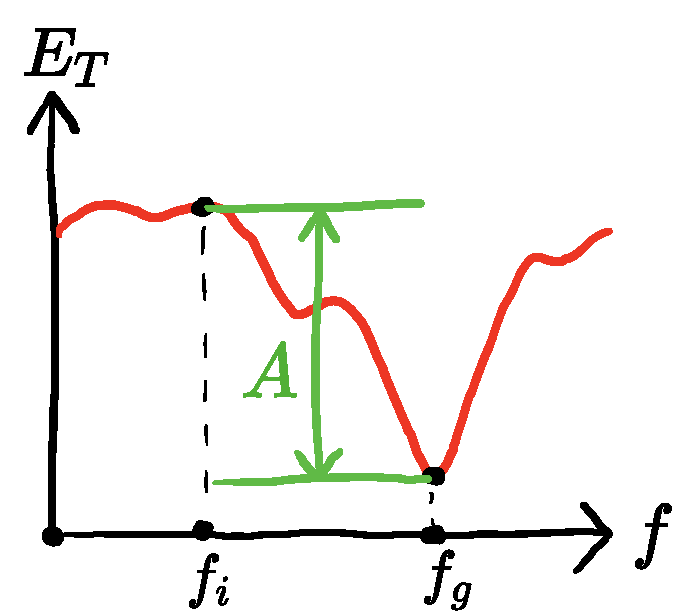
\includegraphics[width=0.5\textwidth]{3_chapters/0_introduction/img/AE-def.pdf}
    \caption{A pictorial representation of the \AE{}. The $x$ axis contains the distribution functions $f \in \mathcal{F}_L$, and the $y$ axis is their associated thermal energy. The initial distribution function is denoted by $f_i$ and the ground state is denoted by $f_g$. Finally, the available energy is denoted in green as $A$.}
    \label{fig: ae def}
\end{figure}
We finally include a pictorial representation of the \AE{} in Fig. \ref{fig: ae def}, where one can see that the \AE{} is defined as the difference in energy between the initial distribution function and the ground state.
\subsection{History \& development of the concept}
The concept of \AE{} and its mathematical equivalents have been known since 1930. In that year, \citet{riesz1930inegalite} employed an equivalent concept to derive certain integral inequalities, and such Riesz–Sobolev inequalities remain an active field of mathematical research \cite{burchard1996cases,burchard2006rearrangement,hajaiej2011necessity,carlen2017stability,frank2019proof}. The concept first entered the field of physics in 1955, where \citet{lorenz1955available} calculated the \AE{} of the atmosphere under an adiabatic rearrangement. Eight years later, \citet{gardner1963bound} recognised the relevance of such concepts for plasma physics and derived the \AE{} of a collisionless plasma. It will be of interest to note that Gardner's research focused on the \AE{} of a plasma that is subject to Liouville's theorem {\it alone,} i.e. there are no additional constraints on the system. Gardner was acutely aware of this important distinction, as he explicitly points it out in the abstract of his aforementioned paper. \par 
Though this distinction was recognised in 1963 by Gardner, it was \citet{helander2017available,helander2020available} who recognised its significance in 2017. By allowing additional constraints on the set of accessible distribution functions, the \AE{} becomes relevant to magnetically confined plasmas, as such plasmas do not obey Liouville's theorem alone; they have additional {\it adiabatic invariants.} If we denote an additional set of conserved invariants by $\boldsymbol{y}$, the set of accessible distribution functions is thus reduced by constancy of these invariants, and this set shall be denoted by $\mathcal{F}_L[f_i;\boldsymbol{y}]$.\footnote{Note that $\mathcal{F}_L[f_i;\boldsymbol{y}] \subseteq \mathcal{F}_L[f_i]$, which implies that the \AE{} with constancy of adiabatic invariants is smaller than or equal to the \AE{} without such constancy.} Helander employed an elegant scheme (involving Lagrange multipliers) to find the ground-state of such plasmas, and was able to reproduce many known results from the literature. \par 
All mentioned research has relied heavily on Liouville's theorem, and it is natural to wonder how breaking of this theorem affects \AE{}. It, very surprisingly, turns out that \AE{} in continuous systems that allow for phase-space mixing is the \textit{same} as in systems in which Liouville's theorem is obeyed, as proven in \citet{kolmes2020recovering} in 2020. In terms of collisionality, \AE{} is thus unchanged as the collision frequency increases given that the adiabatic invariants $\boldsymbol{y}$ remain conserved. There is an additional question, pertaining to accessibility of the ground state. That is, though the ground state is within the set of distribution functions obeying certain conditions, it is not guaranteed that the ground state is {\it dynamically accessible,} and some comments relating to dynamical accessibility of ground states may be found in \citet{ewart2022collisionless}.\footnote{In general one should not expect the ground state to be accessible (best surmised by A. Schekochihin, who during a talk cleverly remarked \textit{``the bound is bound not to be sharp''}). This is because we have not imposed that this ground state supports an electromagnetic field which has the appropriate magnitude. This ailment can be remedied, and in simplified scenarios, this difference turns out to be minute. More general scenarios are still being considered in a collaboration with R.J. Ewart} More generally, since it is unknown whether the state is accessible \textit{a priori} one can best interpret \AE{} as an upper bound of the amount of liberated thermal energy. 
\section{Research question \& contributing works}
Given the generality of the concept of \AE{}, it is somewhat surprising that it has found fairly little use as a practical tool to study gyrokinetic turbulence in fusion reactors. This is especially true given the fact that \AE{} possesses the following attractive properties:
\begin{enumerate}
    \item It provides a natural mapping from the magnetic geometry of the device (i.e. the shape of the flux-surfaces) and the plasma profiles (e.g. pressure and temperature) to a scalar. This allows one to condense the large parameter space of fusion reactors into a physically meaningful quantity.
    \item Although the calculation of \AE{} in the most general case is not trivial, it can be significantly faster than the gyrokinetic codes. This is partly a consequence of the fact that \AE{} is not a dynamical quantity; there is no time-stepping involved.
    \item Vanishing \AE{} (that is, $A = 0$) implies \textit{ nonlinear} stability. Thus, it is natural to quantify the distance from such stability thresholds.
\end{enumerate}
We note in passing that these factors not only make \AE{} interesting as a measure of turbulence but also make it interesting as an optimisation measure. Overall, given the broad applicability and relatively unexplored use of \AE{} in gyrokinetic turbulence, the central idea of the current thesis is the following:
\boxedtext{Can \AE{} predict gyrokinetic turbulent transport and can it be used to infer its dependencies?}

Since \AE{} is very broadly applicable, we choose to specialise in trapped-electron-mode driven turbulence first, and its corresponding \AE{}. As it turns out, many quantities signifying trapped particles will enter into the calculation of the \AE{}, and we first develop numerical methods of evaluating these quantities efficiently, which is the first contribution of this thesis.
\itemheader{Bounce-averaged drifts: equivalent definitions, numerical implementations, and example cases}
\textit{Abstract:} In this paper, we provide various analytical and numerical methods for calculating the average drift of magnetically trapped particles across field lines in complex geometries, and we compare these methods with each other. To evaluate bounce-integrals, we introduce a generalisation of the trapezoidal rule, which is able to circumvent integrable singularities. We contrast this method with more standard quadrature methods in a parabolic magnetic well and find that the computational cost is significantly lower for the trapezoidal method, though at the cost of accuracy. With numerical routines in place, we next investigate conditions on particles which cross the computational boundary, and we find that important differences arise for particles affected by this boundary, which can depend on the specific implementation of the calculation. Finally, we investigate the bounce-averaged drifts in the optimized stellarator NCSX. From investigating the drifts, one can readily deduce important properties, such as what subset of particles can drive trapped-particle modes, and in what regions radial drifts are most deleterious to the stability of such modes.
\contribution{Develop new numerical methods for evaluating the bounce-averaged drift, and develop benchmark cases to test them on. Finally, recognize that the computational boundary may affect the trapped-particle drift in non-trivial ways.}{\label{contr:BAD}} \par 
The second contribution employs these numerical methods to find the \AE{} of trapped electrons. To this end, we derive the \AE{} of trapped electrons to non-omnigenous systems, which generalizes results found in \citet{helander2020available}, and we go on to investigate it in some depth. Importantly, we compare \AE{} against the nonlinear heat-flux, an important measure for turbulence in magnetic confinement fusion reactors. 
\itemheader{The available energy of trapped particles and its relation to turbulent transport} \\
\textit{Abstract:} A collisionless plasma possesses a certain amount of ``available energy'', which is that part of the thermal energy that can be converted into kinetic energy of plasma motion and electromagnetic fluctuations. In this paper we present a calculation of the available energy carried by trapped electrons in a slender non-omnigenous flux tube of plasma. This quantity is compared with gyrokinetic simulations of the nonlinear saturated radial energy flux resulting from turbulence driven by collisionless trapped-electron modes in various stellarators and a tokamak. The numerical calculation of available energy is fast and shows a strong correlation with the turbulent energy fluxes found in the gyrokinetic simulations. Indeed, the energy flux is found to be proportional to the available energy to the power of approximately $3/2$, which is what one would expect from a simple argument. We furthermore investigate how available energy is distributed across different bounce wells, and it is found that deeply trapped electrons typically contribute most to the available energy. Finally, we investigate the dependence of available energy on gradient strength, and we find important differences between weakly and strongly driven regimes for stellarators and tokamaks.
\contribution{Generalize the \AE{} of trapped particles to account for non-omnigenous systems. Develop numerical routines to calculate the \AE{}. Relate \AE{} to turbulent transport. Investigate which regions are most unstable, and investigate how the \AE{} changes with gradient strengths.}{\label{contr:AE-and-turbulence}}

Seeing the found utility of the \AE{} of trapped electrons, we go on to specialise to tokamaks, which we parameterize via the Miller equilibrium \cite{miller1998noncircular}. The model allows us to make statements about the possible benefits and disadvantages of negative triangularity tokamaks, which have found renewed interest after having shown improved confinement in such cases \cite{marinoni2021brief}. Triangularity is a measure in tokamaks of how triangular the flux-surfaces are, and negative/positive triangularity have the triangle pointing towards/away from the center of the torus. We go in to investigate how \AE{} against a number of other equilibrium parameters, and find that it is able to reproduce many trends.

\itemheader{Available energy of trapped electrons in Miller
tokamak equilibria} \\
\textit{Abstract:} Available energy (\AE{}), which quantifies the maximum amount of thermal energy that may be liberated and converted into instabilities and turbulence, has shown to be a useful metric for predicting saturated energy fluxes in trapped-electron-mode-driven turbulence. Here, we calculate and investigate the \AE{} in the analytical tokamak equilibria introduced by \citet{miller1998noncircular}. The \AE{} of trapped electrons reproduces various trends also observed in experiments; negative shear, increasing Shafranov shift, and negative triangularity can all be stabilizing as indicated by a reduction in \AE{}, though it is strongly dependent on the chosen equilibrium. We find that negative triangularity is especially beneficial in vertically elongated configurations with positive shear, or low gradients. We furthermore extract a gradient-threshold like quantity from \AE{} and find that it behaves similarly to gyrokinetic gradient-thresholds: it tends to increase linearly with magnetic shear, and negative triangularity leads to an especially high threshold. We next optimize device geometry for minimal \AE{} and find that the optimum is strongly dependent on equilibrium parameters. If one furthermore investigates the competing effects of increasing the density gradient, pressure gradient, and decreasing the shear, one finds regimes which have steep gradients yet low \AE{}, and that the existence of such a regime is inaccessible in negative-triangularity tokamaks. We finally compare \AE{} with saturated heat-flux estimates from the \textsc{tglf} model and find fairly good correspondence.

\contribution{Investigate possible benefits/disadvantages of negative triangularity. Find dependencies of an critical gradient-like quantity in \AE{}. Research how geometrically \AE{}-optimized tokamaks depend on equilibrium parameters. Investigate how \AE{} differs as one enters a pedestal-like regime. Finally, compare against \AE{} against heat-fluxes from \textsc{tglf}.}

\section{Outline of the thesis}
[To be filled in after finalisation of the structure.]
% \section{Scrap}
% \label{sec: chap1 contributions}

% Supposing that one parameterizes phase-space by the coordinates $\boldsymbol{x}$, which furthermore have the Jacobian $\sqrt{g}$, the continuity equation for the particle distribution function becomes
% \begin{equation}
%     \frac{\partial (f\sqrt{g})}{\partial t} + \dot{\boldsymbol{x}} \cdot  \nabla_{\boldsymbol{x}} (f\sqrt{g}) = 0.
%     \label{eq: continuity equation in general}
% \end{equation}
% Now, phase-space incompressibility implies that the Jacobian obeys
% \begin{equation}
%     \frac{\partial \sqrt{g}}{\partial t} + \dot{\boldsymbol{x}} \cdot \nabla_{\boldsymbol{x}} \sqrt{g} = 0.
%     \label{eq: Liouville theorem for Jacobian}
% \end{equation}
% Combining Eqs. \eqref{eq: continuity equation in general} and \eqref{eq: Liouville theorem for Jacobian}, we find
% \begin{equation}
%     \frac{\partial f}{\partial t} + \dot{\boldsymbol{x}} \cdot \nabla_{\boldsymbol{x}} f = 0.
% \end{equation}
% If we now multiply the above equation by some function $G'[f]$, use the chain rule, and finally integrate over $\boldsymbol{x}$, one finds
% \begin{equation}
%     \frac{\mathrm{d}}{\mathrm{d} t} \int G[f] \mathrm{d} \boldsymbol{x} = 0 \longrightarrow \int G[f] \mathrm{d} \boldsymbol{x} = \mathrm{const.}
%     \label{eq: constraints G[f]}
% \end{equation}
% Eq. \eqref{eq: constraints G[f]} puts an uncountably infinite number of constraints on $f$, as we may choose any well-behaved function $G[f]$. In essence, this equation describes Liouville's theorem from the perspective of the distribution function: since phase-space flow is incompressible, the set of all $f$ is heavily constrained. To gain some insight we parameterize the functions $G[f]$ as
% \begin{equation}
%     G[f] = H[f-\phi]; \quad \forall \phi \in \mathbb{R},
% \end{equation}
% where $\phi$ is some scalar constant and $H[x]$ is the Heaviside function of $x$. To aid notation, denote this constrained subset of distribution functions as $\mathcal{F}[f_i]$ where the member distribution functions $f$ of this set are defined by
% \begin{equation}
%     \int H[f - \phi] \mathrm{d} \boldsymbol{x} = \int H[f_i-\phi]\mathrm{d} \boldsymbol{x} ; \; \forall \phi \in \mathbb{R} \iff f \in \mathcal{F}[f_i].
% \end{equation}
% Here $f_i\equiv f(t=0,\boldsymbol{x})$ is the initial condition/distribution function, which determines the set of accessible distribution functions. Summarizing, one finds that, if there is a continuity equation for $f$ with a Liouville theorem, $f \in \mathcal{F}[f_i]$ where $f_i$ is the initial condition. \par 

% Let us use this knowledge to our benefit.

% %**********************************************************************%

% \itemheader{Topic 1}
% \lipsum[1-2] This leads to the first contribution of our work:

% \contribution{First contribution of your work.}{\label{contr: contribution 1}}

% Explain a bit more about your first contribution.

% %**********************************************************************%

% \itemheader{Topic 2}
% \lipsum[4-5] This leads to the second contribution of our work:

% \contribution{Second contribution of your work.}{\label{contr: contribution 2}}

% Explain a bit more about your second contribution.

% %**********************************************************************%

% \itemheader{Topic 3}
% \lipsum[1-2] The last contribution of the research thus is:

% \contribution{Third contribution of your work.}{\label{contr: contribution 3}}

% Explain a bit more about your third contribution.


% \section{Outline of the thesis}
% \label{sec: chap1 outline}

% \lipsum[10-12]

% \itemheaderNewpage{A note for the reader} Chapters~...-... are all based on submitted/published articles and consequently are self-contained and can be read independently. A reference to the corresponding research paper is included at the beginning of each chapter.
% An overview of how the chapters of this thesis relate to the contributions presented in Section~\ref{sec: chap1 contributions} is given in Table~...

